\documentclass[12pt]{article}
\usepackage[utf8]{inputenc}
\usepackage{graphicx}
\usepackage{amsmath}
\usepackage{hyperref}
\usepackage{booktabs}
\usepackage{indentfirst}
\usepackage{float}
\usepackage{geometry}
\geometry{margin=1in}
\usepackage{setspace} % Enables setting line spacing
\setlength{\parindent}{2em} % Sets the indentation size for all paragraphs
\setlength{\parskip}{0em} % Ensures no extra space between paragraphs

% Double-spacing throughout the document
\doublespacing

\title{Survival Analysis of Infection Control Measures in Burn Patients}
\author{Ziyue Yang}
\date{\today}

\begin{document}

\maketitle

\section*{Introduction}

Infection with \textit{Staphylococcus aureus} is a critical concern in burn patients, often contributing to prolonged hospital stays, increased morbidity, and higher healthcare costs \cite{norbury_infection_2016}. Therefore, effective infection control measures are of great importance. This study investigates the impact of replacing routine bathing with total body washing using antimicrobial agents on infection risk, leveraging survival analysis techniques to rigorously evaluate the time to infection. The dataset, originally published by Ichida \textit{et al.} (1993), provides data on infection times, patient characteristics, and clinical interventions \cite{ichida_evaluation_1993}.

To highlight differences in infection-free survival between patients receiving routine bathing and those undergoing total body washing, the Kaplan-Meier estimator was used \cite{kaplan_nonparametric_1958}. 

To further identify factors influencing infection risk, the Cox proportional hazards model was employed \cite{cox1972}. Both time-independent covariates (e.g., patient gender, race) and time-dependent covariates (e.g., surgical excision of burn tissue, prophylactic antibiotic treatment) were analyzed to provide a comprehensive evaluation of \textit{Staphylococcus aureus} infection in burn patients.

This report aims to present a clear and actionable evaluation of the infection control measures through the lens of survival analysis, with insights that inform clinical decision-making and contribute to better patient care.


\section*{Data Description}

The dataset \texttt{burn} consists of 154 observations of burn patients and 17 variables that capture patient characteristics, clinical interventions, and infection status with time to infection.  

\subsection*{Outcome Variables}
\begin{itemize}
    \item \textbf{T3 (time to infection)}: The time (in days) until infection with \textit{Staphylococcus aureus}.
    \item \textbf{D3 (infection status)}: A binary variable indicating whether the patient developed an infection within the course of the study (1 = infected, 0 = not infected).
\end{itemize}

\subsection*{Time-Dependent Covariates}
\begin{itemize}
    \item \textbf{T1 (time to surgical excision)}: The time (in days) to surgical excision of burn tissue.
    \item \textbf{D1 (surgical excision status)}: A binary variable indicating whether surgical excision was performed (1 = excised, 0 = not excised).
    \item \textbf{T2 (time to antibiotic treatment)}: The time (in days) to the administration of prophylactic antibiotic treatment.
    \item \textbf{D2 (antibiotic treatment status)}: A binary variable indicating whether antibiotics were administered (1 = treated, 0 = not treated).
\end{itemize}

\subsection*{Baseline Characteristics}
\begin{itemize}
    \item \textbf{Treatment}: Categorical variable indicating the bathing regimen (Routine or Cleansing with antimicrobial agents).
    \item \textbf{Gender}: Categorical variable indicating the patient's gender (Male or Female).
    \item \textbf{Race}: Categorical variable indicating the patient's race (Nonwhite or White).
    \item \textbf{PercentBurned}: Numeric variable representing the percentage of the patient’s body surface area affected by burns.
\end{itemize}

\subsection*{Burn Site Characteristics}
\begin{itemize}
    \item \textbf{SiteHead}: Binary factor indicating whether the head was burned (Burned or Not Burned).
    \item \textbf{SiteButtock}: Binary factor indicating whether the buttocks were burned (Burned or Not Burned).
    \item \textbf{SiteTrunk}: Binary factor indicating whether the trunk was burned (Burned or Not Burned).
    \item \textbf{SiteUpperLeg}: Binary factor indicating whether the upper leg was burned (Burned or Not Burned).
    \item \textbf{SiteLowerLeg}: Binary factor indicating whether the lower leg was burned (Burned or Not Burned).
    \item \textbf{SiteRespTract}: Binary factor indicating whether the respiratory tract was burned (Burned or Not Burned).
\end{itemize}

\subsection*{Burn Type}
\begin{itemize}
    \item \textbf{BurnType}: Categorical variable specifying the type of burn (Chemical, Scald, Flame, or Electric).
\end{itemize}

\section*{Methods}

\subsection*{Kaplan-Meier Survival Analysis}

The Kaplan-Meier estimator was used to estimate and visualize the probability of remaining infection-free over time for patients undergoing either routine bathing or antimicrobial washing. Additionally, the Nelson-Aalen estimate was plotted for a comprehensive view of survival differences between groups. 

Survival curves were compared using the \texttt{survdiff} function from the \texttt{survival} package in R, which performs a log-rank test to assess whether the differences between the two groups are statistically significant. 

Cumulative hazard functions were plotted against time to estimate the cumulative infection probability at different time points. Complementary log-log survival curves were plotted against log-transformed time to assess if the ratio of hazard rates between the two treatment groups remains constant over time. 

\subsection*{Cox Proportional Hazards Model}

\subsubsection*{Model with Time-Independent Covariates}

An initial Cox proportional hazards model was constructed using all time-independent covariates to evaluate their relationship with the risk of infection. The primary predictor of interest was \textit{Treatment}. Additional time-independent variables were sequentially introduced into the model.

Model refinement was performed using the \texttt{drop1} function to identify covariates that did not significantly contribute to model performance. Multicollinearity among covariates was assessed using variance inflation factors, ensuring that redundant predictors were identified and addressed without compromising the integrity of the model. The significant time-independent covariates were determined to be \textit{Treatment} and \textit{Race}. 

\subsubsection*{Model with Time-Dependent Covariates}

To incorporate time-dependent predictors, the dataset was expanded using counting process notation. Two key time-dependent covariates were included: Surgical excision of burn tissue (T1, D1) and Prophylactic antibiotic treatment (T2, D2).

A Cox model was constructed upon the chosen time-independent covariates with time-dependent covariates. The time-dependent variables captured the dynamic effects of these interventions on infection risk, while time-independent variables provided baseline hazard adjustments.

\subsection*{Model Checking and Diagnostics}

\subsubsection*{Proportional Hazards Assumption}

The proportional hazards assumption was evaluated using Schoenfeld residual plots, which test whether the residuals show systematic trends over time, and the \texttt{cox.zph} function from the \texttt{survival} package. Where violations were detected, appropriate adjustments were made, such as stratification to allow baseline hazard functions to differ between groups. According to both Schoenfeld residual plots (Fig. 1) and the \texttt{cox.zph} function output (Table 1), no violation of the proportional hazards assumption was found. 

\begin{figure}[H]
    \centering
    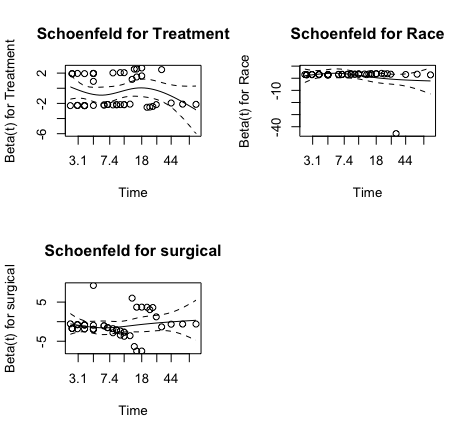
\includegraphics[width=0.8\textwidth]{plots/schoenfeld.png}
    \caption{\textbf{Schoenfeld residual for Treatment, Race, and Excision Surgery. } All three curves look about flat, indicating no significant violation of the proportional hazards assumption. }
    \label{fig:km_na_curves}
\end{figure}

\begin{table}[H]
\centering
\caption{\textbf{Schoenfeld Residual Test for Proportional Hazards Assumption}}
\label{tab:cox_zph}
\begin{tabular}{lccc}
\toprule
Variable   & Chi-square (\( \chi^2 \)) & Degrees of Freedom (df) & \( p \)-value \\
\midrule
Treatment  & 0.296                     & 1                       & 0.59          \\
Race       & 2.162                     & 1                       & 0.14          \\
Surgical   & 0.516                     & 1                       & 0.47          \\
\textbf{Global} & 3.052                     & 3                       & 0.38          \\
\bottomrule
\end{tabular}
\end{table}


\subsubsection*{Goodness-of-Fit}

Cox-Snell residuals were used to assess overall model fit. A cumulative hazard plot was constructed to compare observed data with the expected hazard under the model. A straight 45-degree line indicated good fit, while deviations suggested potential inadequacies. According to Fig. 2, 

\begin{figure}[H]
    \centering
    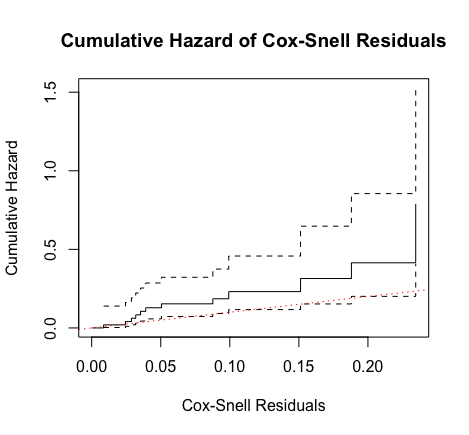
\includegraphics[width=0.8\textwidth]{plots/cox_snell.png}
    \caption{\textbf{Cumulative Hazard of Cox-Snell Residuals.} The reference line lies within the 95\% confidence interval, suggesting a reasonable good fit. }
    \label{fig:km_na_curves}
\end{figure}


\subsubsection*{Outlier Analysis}

Residual analysis was performed to evaluate how well the Cox model aligned with the observed data and to identify unusual observations. Two types of residuals -- deviance residuals and DFBETA values -- were analyzed. 

Martingale residuals (Fig. 3) were not analyzed in this study due to their limitations in evaluating model adequacy for survival data. While martingale residuals can be useful for assessing the functional form of covariates, they are heavily skewed, especially for censored data, making interpretation challenging.  Instead, deviance residuals (Fig. 4), which are transformations of martingale residuals, were used to identify discrepancies between observed and predicted infection times. Deviance residuals measure how much an individual’s observed time to infection deviates from the model’s prediction, with positive values indicating later-than-expected infections. 

\begin{figure}[H]
    \centering
    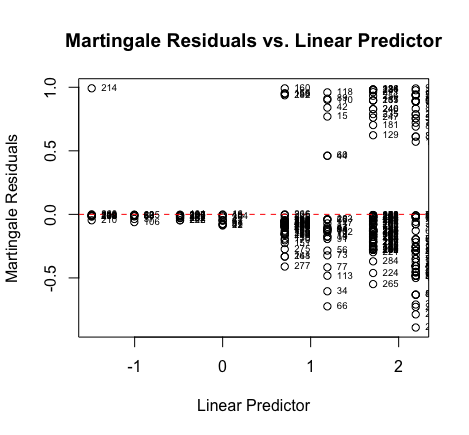
\includegraphics[width=0.8\textwidth]{plots/martingale.png}
    \caption{\textbf{Martingale Residuals vs. Linear Predictor.} Most Martingale residuals cluster around 0, but observations with martingale close to 1 exists. In particular, Obs 214, 160 need further investigation because of their high residual value. }
    \label{fig:km_na_curves}
\end{figure}

\begin{figure}[H]
    \centering
    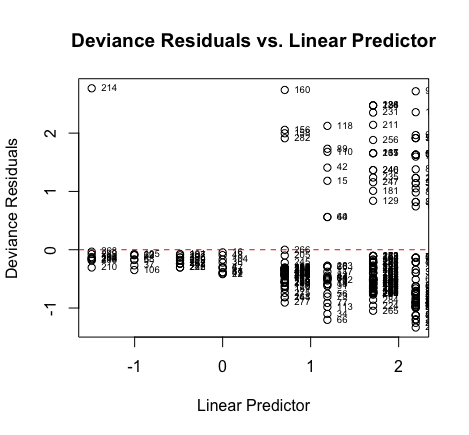
\includegraphics[width=0.8\textwidth]{plots/deviance.png}
    \caption{\textbf{Deviance Residuals vs. Linear Predictor.} Most Deviance residuals cluster between -1 and 0, but observations with extreme deviance residual around 2 such as 214, 160, etc. needs further investigation. }    
    \label{fig:km_na_curves}
\end{figure}

DFBETA values (Fig. 5) measure the influence of individual observations on the model’s coefficients. Large DFBETA values indicate that a specific observation has a strong effect on a particular predictor. 

\begin{figure}[H]
    \centering
    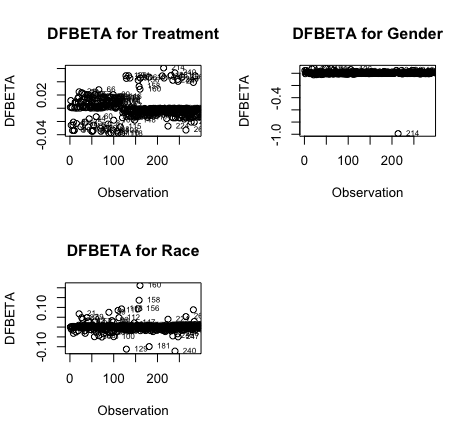
\includegraphics[width=0.8\textwidth]{plots/dfbeta.png}
    \caption{\textbf{DFBETA Calue vs. Observation Index. } In DFBETA for treatment, Obs 214 stands out with a high DFBETA value. In DFBETA for Gender, Obs 214 stands out with an extremely low DFBETA value. In DFBETA for Race, Obs 160 and 158 stand out with high DFBETA value, and Obs 129, 181, and 240 needs more investigation because of their low DFBETA value.}
        \end{figure}

\section*{Result and Discussion}
\subsection*{Kaplan-Meier and Nelson-Aalen Analysis}

Fig. 1 illustrates differences in infection-free survival between routine care and antimicrobial cleansing. After 30 days, 76\% of patients in the cleansing group remained infection-free compared to 66\% in the routine care group. By the end of the study, 70\% of cleansing patients remained infection-free, compared to 30\% in the routine care group. 

The Nelson-Aalen curves confirmed these trends, showing slightly higher infection-free percentages for both groups. The survival curves do not cross, suggesting that the relative risk between the two treatment groups remains constant over time.

\begin{figure}[H]
    \centering
    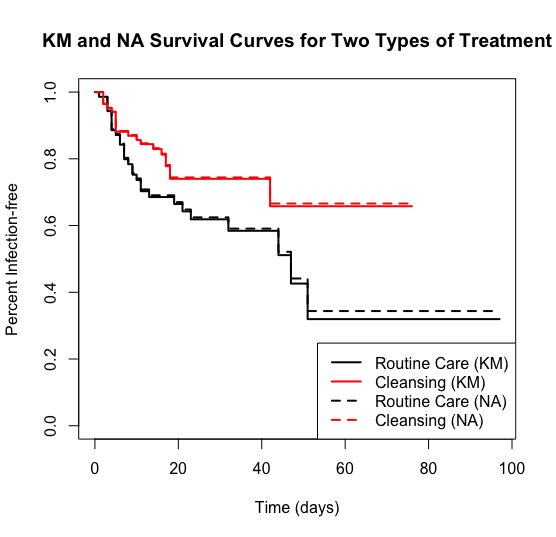
\includegraphics[width=0.8\textwidth]{plots/km_na_curve.png}
    \caption{Kaplan-Meier and Nelson-Aalen Survival Curves. 
    Both Kaplan-Meier (solid line) and Nelson-Aalen (dashed line) curves illustrate the proportion of patients remaining infection-free over time for routine care (black) and antimicrobial cleansing groups (red). Patients receiving antimicrobial cleansing consistently showed higher infection-free survival rates compared to routine care throughout the study.}
    \label{fig:km_na_curves}
\end{figure}

The log-rank test supports the observed differences in survival (\( \chi^2 = 3.8 \)), with a borderline p-value of 0.05. Patients in the antimicrobial cleansing group experienced fewer observed infections (20) than expected (26.6), while those in the routine care group experienced more infections (28) than expected (21.4). These results suggest that antimicrobial cleansing offers a protective benefit in reducing infection risks.


\subsection*{Cox Proportional Hazards Model}

The final Cox proportional hazards model is given by the following equation for the hazard function:

\[
h(t | X) = h_0(t) \cdot \exp\left(-0.4843 \cdot \text{Trt} + 2.1939 \cdot \text{Race} - 1.0039 \cdot \text{Surg}\right)
\]

Where:
\begin{itemize}
    \item \( h(t | X) \): Hazard function conditional on covariates.
    \item \( h_0(t) \): Baseline hazard function (unspecified).
    \item \(\text{Trt} = 1\) for cleansing treatment, \(0\) for routine care.
    \item \(\text{Race} = 1\) for White patients, \(0\) for non-White patients.
    \item \(\text{Surg} = 1\) if surgical excision was performed, \(0\) otherwise.
\end{itemize}

Specifically, patients receiving antimicrobial cleansing were 40.4\% less likely to develop an infection compared to those in the routine care group (\(p = 0.082\)). While not statistically significant, this result suggests a potential protective effect that warrants further validation. White patients were significantly more likely to develop an infection compared to non-White patients, with an 8.86-fold higher likelihood of infection (\(p = 0.031\)). The wide confidence interval (95\% CI: 1.22–64.34) reflects uncertainty due to the small sample size (\(n = 154\)). Surgical excision was associated with a 60\% lower likelihood of infection (\(p = 0.059\)), indicating a marginally significant effect.

The proportional hazard assumptions were met, 



The model demonstrated good predictive performance, with a concordance index of 0.696, correctly predicting the order of infection risk in approximately 69.6\% of cases. The likelihood ratio test confirmed the statistical significance of the model (\(p = 0.0004\)).

\subsection*{Residual Analysis}

Analysis of deviance residuals revealed several cases where the observed time to infection deviated significantly from the model’s predictions. A positive deviance residual indicates that the infection occurred later than predicted, while a negative residual suggests earlier infection.

For example, observation 65 is a white male with 85\% burns on the head, buttocks, trunk, upper leg, and respiratory tract who received routine care had a deviance residual of 2.36, indicating later-than-expected infection. In addition, observation 15 is a white male with 20\% burns on the head and trunk who received routine care, no excision surgery, and no antibiotics had a deviance residual of -1.33, indicating earlier-than-expected infection. Table 1 shows the patient characteristics of high deviance residual individuals (\( > 2\text{SD} \)) that might worth further investigations.

\begin{table}[H]
\centering
\caption{Extreme Observations with High Deviance Residuals}
\label{tab:extreme_deviance}
\begin{tabular}{lllllllll}
\toprule
Obs & Gender & Race      & \% Burned & Treatment   & Surgical & Antibiotics & Deviance \\
\midrule
58  & Male   & White     & 3         & Routine     & 0        & 0           & 2.718    \\
65  & Male   & White     & 85        & Routine     & 0        & 1           & 2.359    \\
70  & Female & White     & 36        & Routine     & 1        & 1           & 2.124    \\
75  & Male   & White     & 5         & Cleansing   & 0        & 0           & 2.476    \\
79  & Female & White     & 9         & Cleansing   & 0        & 0           & 2.476    \\
90  & Female & White     & 45        & Cleansing   & 1        & 1           & 2.056    \\
92  & Male   & White     & 5         & Cleansing   & 1        & 0           & 2.740    \\
115 & Male   & White     & 50        & Cleansing   & 0        & 0           & 2.142    \\
116 & Male   & Nonwhite  & 20        & Cleansing   & 1        & 1           & 2.769    \\
125 & Male   & White     & 13        & Cleansing   & 0        & 1           & 2.352    \\
153 & Male   & White     & 10        & Cleansing   & 0        & 0           & 2.476    \\
\bottomrule
\end{tabular}
\end{table}


Large DFBETA values identified influential observations. For instance: observation 91 is a white male with 20\% burns who received cleansing care, excision surgery, and antibiotics had a high influence on the time-dependent covariate \textit{surgery} with a DFBETA value of 0.137. Observation 92 is a white male with 5\% burns who received cleansing care and excision surgery had a high influence on the \textit{surgery} coefficient with a DFBETA value of 0.212, and also a high deviance residual.


\section*{Conclusion}

In conclusion, the risk of infection was 40.4\% lower in patients receiving antimicrobial cleansing, although this result was not statistically significant. Surgical excision also showed a marginally significant protective effect. The findings highlight the potential of antimicrobial cleansing and surgical excision as effective interventions for infection control in burn patients. However, the study's observational design and small sample size limit causal interpretation. Further randomized studies are recommended to validate these results and better inform clinical decision-making.


\bibliographystyle{plain}
\bibliography{bibliography.bib}

\end{document}
